\begin{question}
\noindent Two petri dishes used in a school science lab are mathematically similar circular cylinders, dish $P$ and dish $Q$, as shown below.

\begin{center}
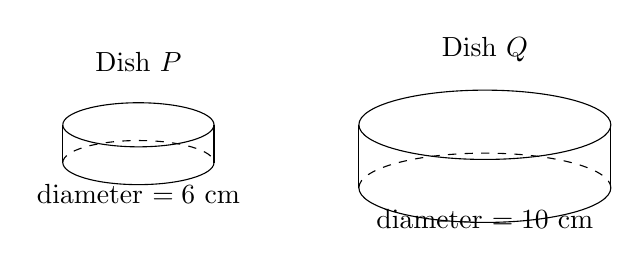
\begin{tikzpicture}[scale=0.8]
    % Dish P (smaller)
    \draw (0,0) ellipse (1.2 and 0.35);
    \draw (-1.2,0) -- (-1.2,-0.6);
    \draw (1.2,0) -- (1.2,-0.6);
    \draw (-1.2,-0.6) arc (180:360:1.2 and 0.35);
    \draw[dashed] (-1.2,-0.6) arc (180:0:1.2 and 0.35);
    \node at (0,1) {Dish $P$};
    \node at (0,-1.1) {diameter $= 6$ cm};

    % Dish Q (larger)
    \begin{scope}[xshift=5.5cm]
        \draw (0,0) ellipse (2 and 0.55);
        \draw (-2,0) -- (-2,-1);
        \draw (2,0) -- (2,-1);
        \draw (-2,-1) arc (180:360:2 and 0.55);
        \draw[dashed] (-2,-1) arc (180:0:2 and 0.55);
        \node at (0,1.2) {Dish $Q$};
        \node at (0,-1.5) {diameter $= 10$ cm};
    \end{scope}
\end{tikzpicture}
\end{center}

\noindent Dish $P$ has a diameter of 6 cm and a total surface area of 84.8 cm$^2$.

\noindent Dish $Q$ is mathematically similar to dish $P$ and has a diameter of 10 cm.

\noindent Work out the total surface area of dish $Q$.

\vspace{5cm}

\begin{flushright}
    \answerunit{$\text{cm}^2$}{3}
\end{flushright}
\end{question}
